                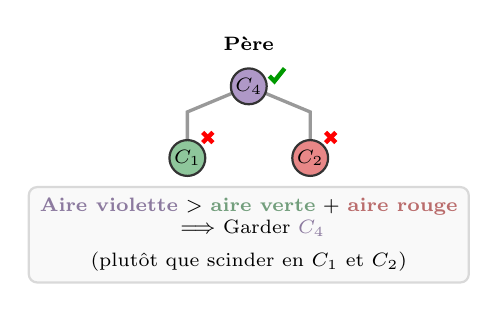
\begin{tikzpicture}[scale=0.65, >=latex, font=\scriptsize]
                    \definecolor{c1}{RGB}{142, 198, 155} % Green
                    \definecolor{c2}{RGB}{232, 135, 135} % Red
                    \definecolor{c4}{RGB}{175, 152, 199} % Violet
                    
                    % Branches
                    \draw[very thick, black!40] (0.8, 0.5) -- (0.8, 1.4) -- (2.0, 1.9) -- (3.2, 1.4) -- (3.2, 0.5);
                    
                    % Nodes
                    \fill[c4, draw=black!80, thick] (2.0, 1.9) circle (0.35) node[black] {$C_4$};
                    \fill[c1, draw=black!80, thick] (0.8, 0.5) circle (0.35) node[black] {$C_1$};
                    \fill[c2, draw=black!80, thick] (3.2, 0.5) circle (0.35) node[black] {$C_2$};
                    
                    % Labels
                    \node[above=3pt] at (2.0, 2.25) {\textbf{Père}};
                    \node[below=3pt] at (0.8, 0.15) {\textbf{Fils 1}};
                    \node[below=3pt] at (3.2, 0.15) {\textbf{Fils 2}};
                    
                    % Checkmark next to C4
                    \draw[green!60!black, ultra thick] (2.4, 2.1) -- ++(0.1, -0.1) -- ++(0.2, 0.25);
                    
                    % Crosses next to C1 and C2
                    \draw[red, ultra thick] (1.1, 0.8) -- ++(0.2, 0.2);
                    \draw[red, ultra thick] (1.3, 0.8) -- ++(-0.2, 0.2);
                    
                    \draw[red, ultra thick] (3.5, 0.8) -- ++(0.2, 0.2);
                    \draw[red, ultra thick] (3.7, 0.8) -- ++(-0.2, 0.2);
                    
                    % Inequality box
                    \node[draw=gray!30, fill=gray!5, rounded corners=3pt, inner sep=4pt, align=center, thick] at (2.0, -1.0) {
                        \textcolor{c4!80!black}{\textbf{Aire violette}} $>$ \textcolor{c1!80!black}{\textbf{aire verte}} $+$ \textcolor{c2!80!black}{\textbf{aire rouge}} \\
                        \vspace{0.1cm}
                        $\Longrightarrow$ Garder \textbf{\textcolor{c4!80!black}{$C_4$}} \\
                        (plutôt que scinder en $C_1$ et $C_2$)
                    };
                \end{tikzpicture}
